\appendix
\setcounter{chapter}{7}
\renewcommand{\thechapter}{\Roman{chapter}.}
\setcounter{section}{7}% Reset numbering for sections
\renewcommand{\thesection}{\arabic{chapter}.\arabic{section}}% Adjust

\chapter[\hspace{0.35cm}ANEXOS]{ANEXOS}
\thispagestyle{empty}
\section*{ANEXO 1: Mapas de la zona de estudio}\appcaption{ANEXO 1: Mapas de la zona de estudio}
...(contents of appendix one)...

\begin{figure}[htbp!]
    \centering
    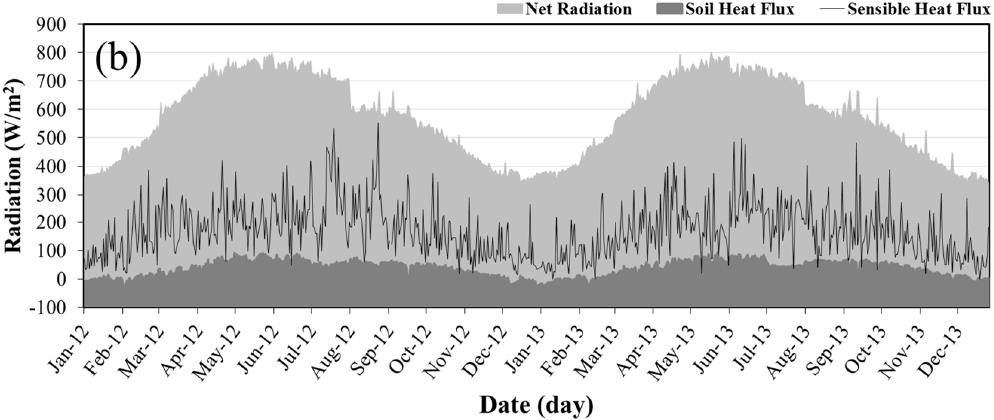
\includegraphics[width=0.9\textwidth]{Figures/f2.png}
    % \addto\captionsspanish{\renewcommand{\appendixname}{Anexo}}
    \caption*{Anexo 1.1: Variación temporal de los componentes del balance energético en la torre de flujo ubicada al centro de arrozales}
    \captionsetup{labelfont=rm,skip=2pt,textfont=rm,font=small}
        \caption*{\textbf{FUENTE:} \parencite{Lee2016}}
    \label{fig:a1}
\end{figure}

\section*{ANEXO 2: Mapas de la zona de estudio}\appcaption{ANEXO 2: Mapas de la zona de estudio}

\section*{ANEXO 3: Mapas de la zona de estudio}\appcaption{ANEXO 3: Mapas de la zona de estudio}

